% METODOLOGIA------------------------------------------------------------------
\chapter{PROCEDIMENTOS METODOLÓGICOS}
\label{chap:metodologia}

Este capítulo tem como finalidade descrever a metodologia e os procedimentos adotados na confecção deste projeto, bem como também realizar uma consolidação de todos os métodos aqui utilizados e apresentar o funcionamento do sistema como um todo. Para tal, os procedimentos metodológicos foram divididos da seguinte forma: Fonte inversora (Seção 3.1), Fonte de alimentação (Seção 3.2),  Realimentação de corrente (Seção 3.3), DSPIC33  (Seção 3.4), Circuito de controle (Seção 3.5), Integração dos componentes (Seção 3.6)

\section{FONTE INVERSORA}
\label{sec:fonteInversora}

Para realizar a alimentação do magnetron, foi utlizada uma fonte inversora, a qual consiste em um inversor ressonanete classe E. Segundo \citeonline{Hidenori1991}, uma fonte inversora tem as seguintes vantagens em relação à uma fonte ferrorressonante tradicional:
\begin{itemize}
    \item Potência de saída controlável;
    \item Maior eficiência energética;
    \item Circuito menor e mais leve;
    \item Pode operar em maior frequência.
\end{itemize} 

\begin{figure}[!htb]
    \centering
    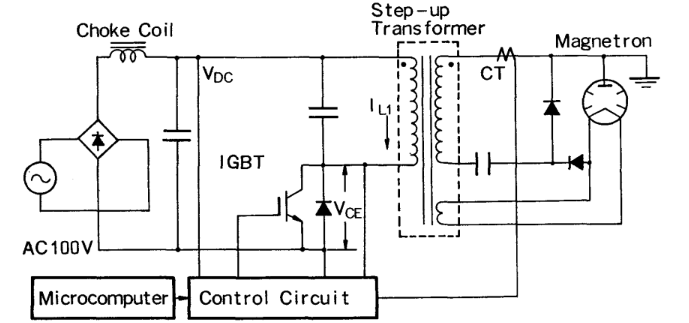
\includegraphics[width=0.9\textwidth]{./dados/figuras/font_inverter}
    \caption{Fonte inversora para alimentação do magnetron}
    \fonte{\citeonline{Hidenori1991}}
    \label{fig:figura-inverter}
\end{figure}

\subsection{Simulações}
\label{sec:simulations}

Para verificar se a fonte inversora é viável para o projeto, foram feitas simulações do circuito no software \textit{PSIM}. Na alimentação o magnetron, são necessários cerca de 4 kV. Assim, primeiramente foi desenvolvido um circuito para simular a alimentação de uma carga de cerca de 100 M$\Omega$, com uma tensão de entrada de 127 V. A figura a seguir mostra o circuito desenvolvido:

\begin{figure}[!htb]
    \centering
    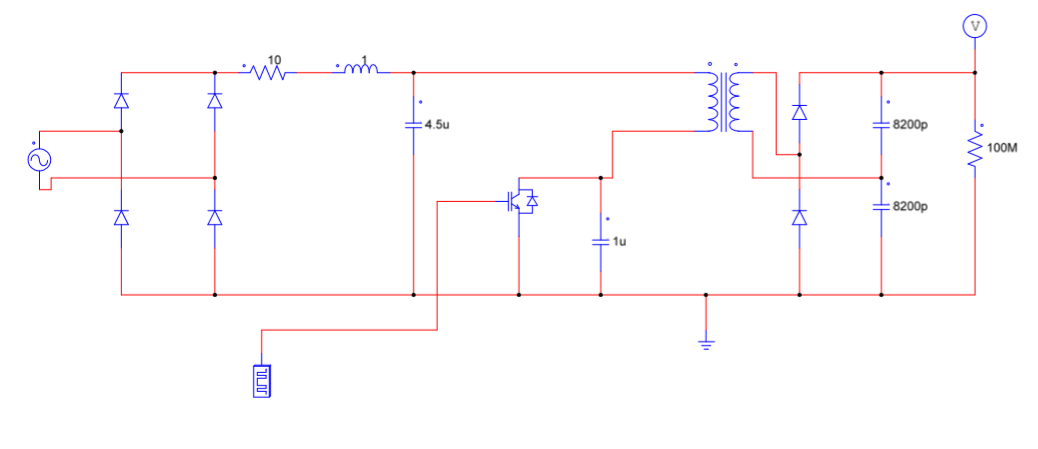
\includegraphics[width=0.9\textwidth]{./dados/figuras/psim1}
    \caption{Circuito da fonte inversora simulada}
    \fonte{Autoria própria (2019)}
    \label{fig:circ_sim_1}
\end{figure}

Para averiguar se uma fonte inversora consegue alimentar uma carga de alta potência à uma tensão de alguns kV, o inversor foi chaveado em um ciclo de trabalho de 50\%. A figura abaixo mostra a froma de onda da tensão na carga resistiva:

\begin{figure}[!htb]
    \centering
    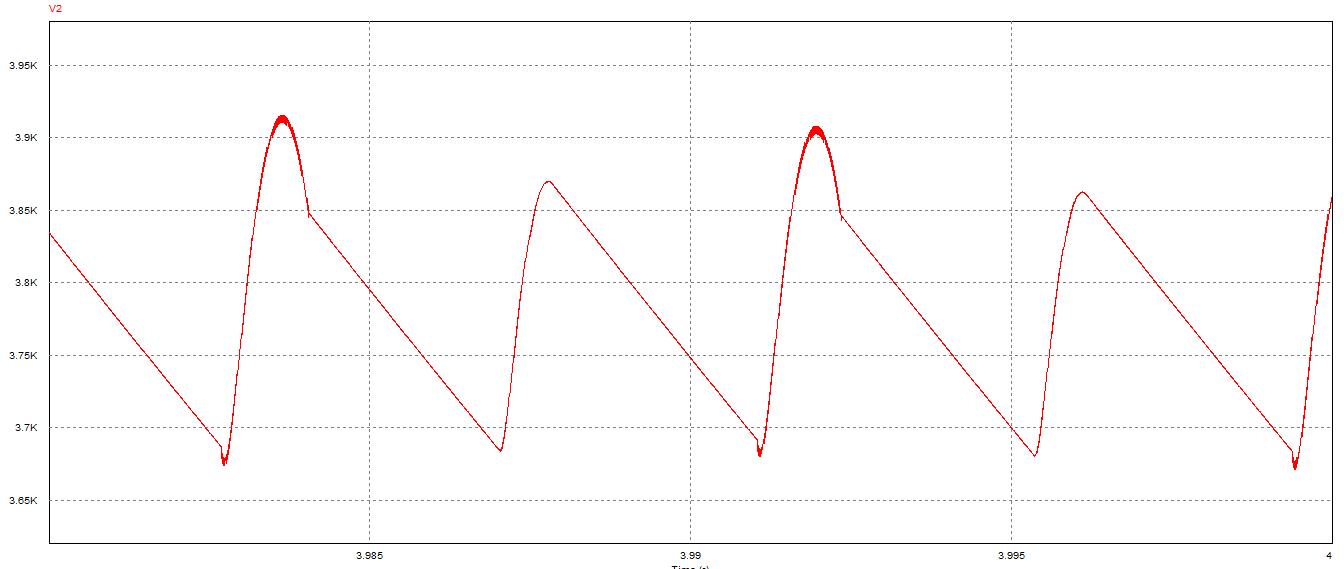
\includegraphics[width=0.9\textwidth]{./dados/figuras/psim2}
    \caption{Forma da onda simulada da tensão na carga}
    \fonte{Autoria própria (2019)}
    \label{fig:figura-graf_sim_1}
\end{figure}

Na figura \ref{fig:figura-graf_sim_1}, pode-se ver que o pico de tensão da carga chega à quase 4 kV, o que já é suficiente para o objetivo em questão. Logo, conclui-se que a fonte inversora é viável para a alimentação do circuito de um magnetron.

\subsection{Projeto}

O projeto da fonte inversora se baseou em boa parte no conceito desenvolvido por \citeonline{Hidenori1991}. Assim como no circuito implementado pelos engenheiros japoneses, a equipe baseou o projeto da fonte em um inversor classe E, e o chaveamento do circuito é feito por um microcontrolador. Devido à operação em alta frequência do sistema, o CI IR1153S foi usado para aplicar uma correção do fator de potência, diminuindo significativamente a taxa de distorção harmônica. Para uma maior eficiência, foram utilizados IGBTs em paralelo para aumentar a potência dos sistemas e reduzir as perdas no circuito. Um transformador de três fios de alta potência alimenta as entradas que são ligadas ao magnetron com uma tensão de cerca de 4kV. A tensão de entrada do circuito é a tensão da rede retificada por uma ponte de diodos. O esquemático do circuito foi desenvolvido no software \textit{Altium Desginer}. A figura \ref{fig:proj-font-inv} mostra o circuito projetado:

\begin{figure}[!htb]
    \centering
    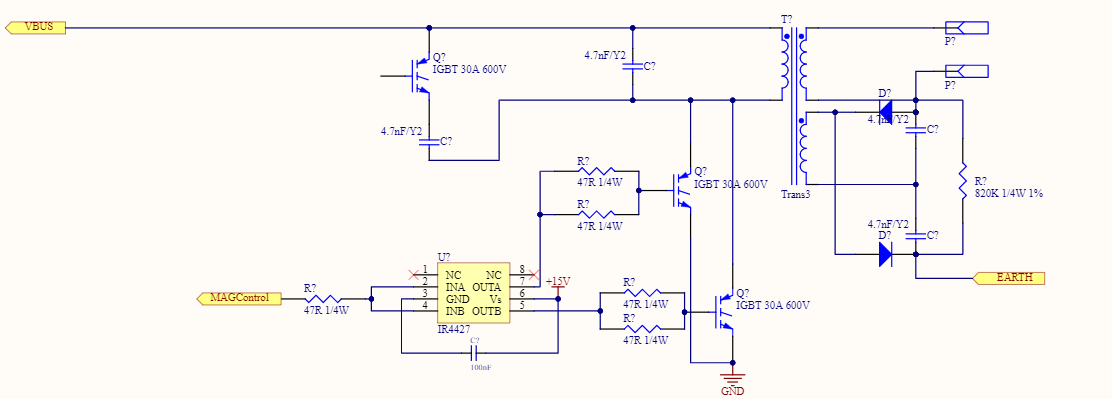
\includegraphics[width=1.1\textwidth]{./dados/figuras/proj-font-inv}
    \caption{Circuito projetado}
    \fonte{Autoria própria (2019)}
    \label{fig:proj-font-inv}
\end{figure}

\subsection{Descrição de funcionamento}

\subsection{Montagem}


\section{\texit{FONTE DE ALIMENTAÇÃO}}
\label{sec:font}

Para alimentar os diferentes componentes do sistema, utilizou-se um projeto de fonte de alimentação isolada, com potência de 10W. A fonte utilizada possui saídas de 3,3V e 15V. A equipe fez uma modificação no circuito para energizar o inversor que faz o controle de potência do magnetron com a tensão após a ponte de diodos. Outra mudança feita foi o posicionamento de um resistor \textit{shunt}, ligado ao neutro do circuito. Este componente atua como um sensor de corrente que é usado na função de transferência da realimentação da planta. A figura abaixo mostra o esquemático da fonte de alimentação utilizada:


\begin{figure}[H]
   \centering
    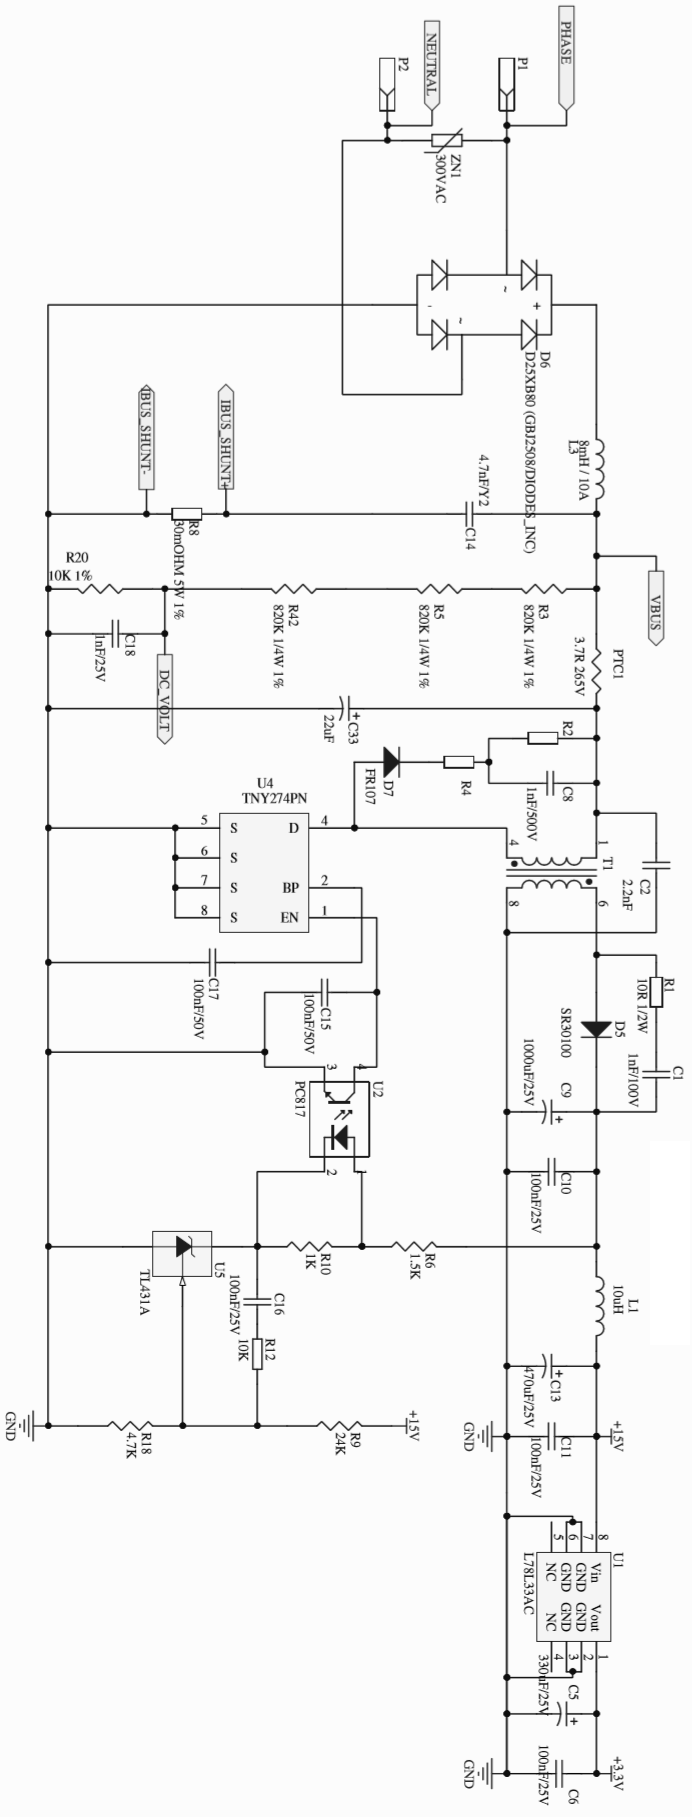
\includegraphics[width=0.55\textwidth]{./dados/figuras/proj-font-alim}
    \caption{Fonte de alimentação do sistema}
    \fonte{Autoria própria (2019)}
    \label{fig:proj-font-inv}
\end{figure}

\pagebreak

\subsection{Montagem}

\section{\texit{REALIMENTAÇÃO DE CORRENTE}}
\label{sec:shunt}
No trabalho apresentado por \citeonline{Hidenori1991}, a planta de controle de potência do magnetron utiliza uma realimentação de corrente, através de um transformador de corrente na saída do secundário do transformador de alta tensão. No entanto, esta abordagem causa distorção no circuito. Como a corrente que circula no sistema está diretamente relacionada à potência fornecida pelo magnetron, a realimentação de corrente foi escolhida como solução, porém a equipe decidiu utilizar uma técnica que utiliza um resistor \textit{shunt}.

 Para possibilitar esta realimentação, foi desenvolvida uma interface analógica que é ligada diretamente ao ADC do microcontrolador. A interface consiste em um circuito que irá condicionar o sinal da tensão aplicada em um resistor \textit{shunt} de 30 m$\Omega$ para os pinos de \textit{input} do microcontrolador. A figura abaixo mostra a interface projetada:

\begin{figure}[!htb]
    \centering
    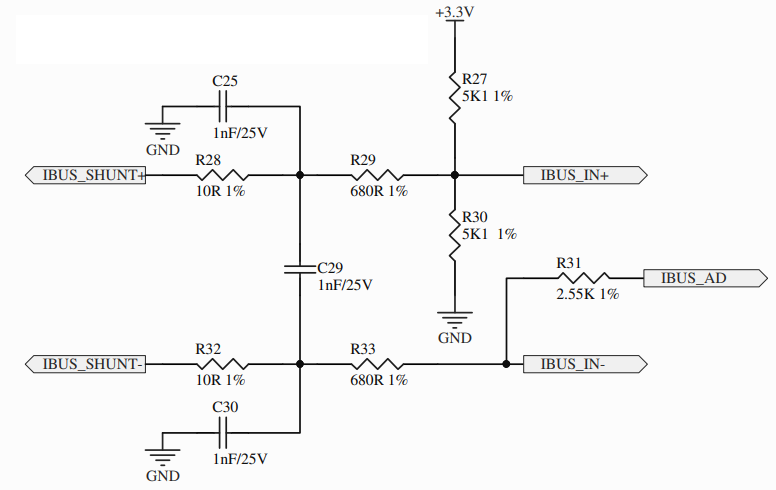
\includegraphics[width=0.9\textwidth]{./dados/figuras/proj-shunt}
    \caption{Condicionador de sinal de realimentação}
    \fonte{Autoria própria (2019)}
    \label{fig:proj-font-inv}
\end{figure}

\subsection{Montagem}

\section{DSPIC33}
\label{sec:dsPIC}

O DSPIC33 é um microntrolador da família PIC, desenvolvido pela Microchip Technology Inc., que possui funcionalidade de processador digital de sinais (DSP). Este componente foi escolhido para fazer o controle do chaveamento da fonte inversora pois consegue operar em uma ampla faixa de temperatura e possui diversas funcionalidades interessantes para o controle de sinais analógicos de alta frequência. Algumas das funcionalidades, cruciais para o projeto, incluem:

\begin{itemize}
    \item Módulo ADC configurável de 10 bits e amostragem de 1.1 Msps ou 12 bits e amostragem de 500 ksps;
    \item Três amplificadores operacionais integrados ao ADC da plataforma;
    \item Interrupções de \textit{Change Notification} em todos os pinos de I/O;
    \item \textit{Timers} e contadores de 32 bits;
    \item Funções de PWM de alta velocidade.
\end{itemize} 

\begin{figure}[!htb]
    \centering
    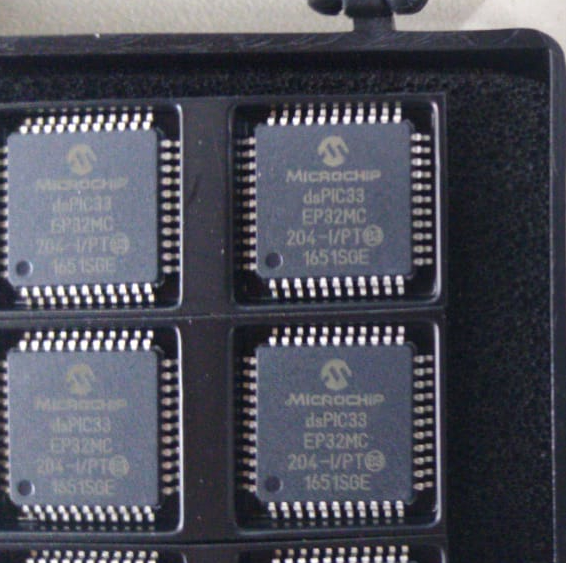
\includegraphics[width=0.3\textwidth]{./dados/figuras/dspic}
    \caption{Microcontrolador DSPIC33}
    \fonte{Autoria própria (2019)}
    \label{fig:figura-dspic}
\end{figure}

A CPU da plataforma possui arquitetura Harvard, típica da família de processadores PIC, possuindo uma palavra de instrução de 24 bits e 12 MB de endereços de memória de programa. O microprocessador possui um extenso suporte ao processamento digital de sinais, tendo acumuladores e ULA de 40 bits, dois multiplicadores de alta velocidade 17 por 17 bits e um \textit{barrell shifter} de 40 bits que consegue alternar 16 bits em úniclo ciclo de \textit{clock}. A arquitetura do processador fornece uma compilação eficiente de código, suportando a linguagem C e \textit{Assembly}.

No circuito, o microcontrolador recebe o sinal de corrente  condicionado dos terminais da interface ligada ao \textit{shunt} e converte este sinal para um valor discreto. No programa do microprocessador, este valor é utilizado no algorítmo de controle, que processa digitalmente o sinal recebido e faz o chaveamento dos IGBTs.

\begin{figure}[H]
    \centering
    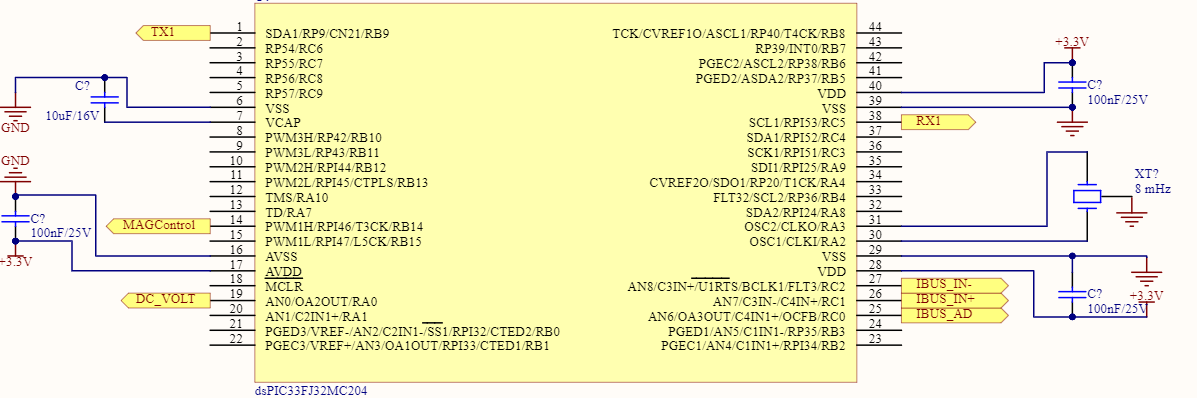
\includegraphics[width=0.9\textwidth]{./dados/figuras/proj-uc}
    \caption{Esquemático do microcontrolador no circuito}
    \fonte{Autoria própria (2019)}
    \label{fig:figura-dspic}
\end{figure}


\section{CIRCUITO DE CONTROLE}
\label{sec:controlCircuit}



\section{INTEGRAÇÃO DOS COMPONENTES}
\label{sec:plant}

